\documentclass[11pt]{article}

% Extract
% \usepackage[active,
%             generate=topology_definitions,
%             %extract-cmd={section},
%             extract-env={definition,algorithm}]{extract}

\usepackage[active,
            generate=topology_theorems,
            %extract-cmd={section},
            extract-env={theorem,corollary,claim}]{extract}

\begin{extract*}

%%%%%%%%%%%%%%%%%%%%%%%%%%%%%%%%%%%%%%%%%%%%%%%%%%%%%%%%%%%%%%%%%%%%%%%%%%%%%%%%%%

% Packages

% AMS 
\usepackage{amsmath, amssymb, amsthm, amsbsy}
% Geometry
\usepackage{geometry}
% Colors
\usepackage[usenames,dvipsnames]{xcolor}
% Figures
\usepackage{graphicx}
\usepackage{float}
% Multi column lists
\usepackage{multicol}
% Subfigures
\usepackage{caption}
\usepackage{subcaption}
% Caligraphic
\usepackage{mathrsfs}
\usepackage{bbm}
% Bold
\usepackage{bm}
% algos
\usepackage[linesnumbered, lined, ruled]{algorithm2e}
% Spacing 
\usepackage{setspace}
% Refs/links
\usepackage[colorlinks=true, citecolor=Blue, linkcolor=blue]{hyperref}
\newcommand\myshade{85}
\colorlet{mylinkcolor}{violet}
\colorlet{mycitecolor}{PineGreen}
\colorlet{myurlcolor}{Aquamarine}

\hypersetup{
  linkcolor  = mylinkcolor!\myshade!black,
  citecolor  = mycitecolor!\myshade!black,
  urlcolor   = myurlcolor!\myshade!black,
  colorlinks = true,
}
% Bibliography
\usepackage{filecontents}
\usepackage{natbib}
% Indent
\usepackage{indentfirst}
% Pretty lists
\usepackage{enumitem}
\setlist[enumerate]{itemsep=2pt,topsep=3pt}
\setlist[itemize]{itemsep=2pt,topsep=3pt}
\setlist[enumerate,1]{label=(\roman*)}

% Code
\usepackage{listings}

% Appendix
\usepackage[toc,page]{appendix}

% Math
\usepackage{mathtools}
\usepackage{xparse}

% Equation numbering
\numberwithin{equation}{section}


%%%%%%%%%%%%%%%%%%%%%%%%%%%%%%%%%%%%%%%%%%%%%%%%%%%%%%%%%%%%%%%%%%%%%%%%%%%%%%%%%%

% Document Settings

% Figure path
\graphicspath{{./figures/}}
% Matrix columns
\setcounter{MaxMatrixCols}{10}
% So pages will break inside long equation environments
\allowdisplaybreaks
% Font
\usepackage{mathpazo} 
\linespread{1.05}  
%\usepackage{courier}
% Geometry
\geometry{left=1in,right=1in,top=1in,bottom=1in}
% Counters
\setcounter{tocdepth}{2}
\setcounter{secnumdepth}{3}

%%%%%%%%%%%%%%%%%%%%%%%%%%%%%%%%%%%%%%%%%%%%%%%%%%%%%%%%%%%%%%%%%%%%%%%%%%%%%%%%%%

% Colors

\definecolor{Tm}{rgb}{0,0,0.80}
\newcommand{\navy}[1]{\textcolor{MidnightBlue}{\bf #1}}

%%%%%%%%%%%%%%%%%%%%%%%%%%%%%%%%%%%%%%%%%%%%%%%%%%%%%%%%%%%%%%%%%%%%%%%%%%%%%%%%%%

% Environments

\theoremstyle{plain}
\newtheorem{theorem}{\color{ForestGreen}{\textbf{Theorem}}}[section]
\newtheorem{claim}{\color{ForestGreen}{\textbf{Claim}}}[section]
\newtheorem{lemma}[theorem]{\color{ForestGreen}{\textbf{Lemma}}}
\newtheorem{proposition}[theorem]{\color{ForestGreen}{\textbf{Proposition}}}
\newtheorem{corollary}[theorem]{\color{ForestGreen}{\textbf{Corollary}}}
\newtheorem{axiom}[theorem]{\color{ForestGreen}{\textbf{Axiom}}}
\newtheorem{conjecture}[theorem]{Conjecture}
\newtheorem{case}[theorem]{Case}
\newtheorem{conclusion}[theorem]{Conclusion}
\newtheorem{criterion}[theorem]{Criterion}
\newtheorem{notation}[theorem]{Notation}
\newtheorem{problem}[theorem]{Problem}

\theoremstyle{definition}
\newtheorem{definition}{\color{MidnightBlue}{\textbf{Definition}}}[section]
\newtheorem{example}{\color{WildStrawberry}Example}[section]
\newtheorem{assumption}{Assumption}[section]
\newtheorem{condition}[assumption]{Condition}
\newtheorem*{solution}{\color{Goldenrod}Solution}
% \newenvironment{solution}[1][\proofname]{%
%   \proof[\bf \color{Goldenrod}Solution to #1]%
% }{\endproof}

\newtheorem{exercise}{\color{YellowOrange}Exercise}[section]

% Literature Summary Standards
\newtheorem*{motivation}{Motivation}
\newtheorem*{summary}{Summary}
\newtheorem*{remark}{Remark}
\newtheorem*{model}{Model}
\newtheorem*{tresults}{Theoretical Results}
\newtheorem*{eresults}{Empirical Results}

%%%%%%%%%%%%%%%%%%%%%%%%%%%%%%%%%%%%%%%%%%%%%%%%%%%%%%%%%%%%%%%%%%%%%%%%%%%%%%%%%%

% Math macros

% Math ``brackets''
\newcommand\parens[1]{\left( #1 \right)}
\newcommand\squares[1]{\left[ #1 \right]}
\newcommand\braces[1]{\left\{ #1 \right\}}
\newcommand\angles[1]{\left\langle #1 \right\rangle}
\newcommand\ceil[1]{\left\lceil #1 \right\rceil}
\newcommand\floor[1]{\left\lfloor #1 \right\rfloor}
\newcommand\abs[1]{\left| #1 \right|}
\newcommand\dabs[1]{\left\| #1 \right\|}
\newcommand\vect[1]{\mathbf{#1}}
\newcommand\closure[1]{\overline{#1}}
\newcommand\pset[1]{\mathcal{P}\left(#1\right)}
\newcommand\inv[1]{#1^{-1}}
\newcommand\norm[1]{\lVert#1\rVert}

% inner product
\providecommand{\inner}[1]{\left\langle{#1}\right\rangle}
% stochastic dominance
\newcommand{\lesd}{\preceq_{\textrm{SD}}}

% Set builder (use \Set ultimately and separate by ;)
\DeclarePairedDelimiterX{\set}[1]{\{}{\}}{\setargs{#1}}
\NewDocumentCommand{\setargs}{>{\SplitArgument{1}{;}}m}
{\setargsaux#1}
\NewDocumentCommand{\setargsaux}{mm}
{\IfNoValueTF{#2}{#1} {#1\nonscript\:\delimsize\vert\allowbreak\nonscript\:\mathopen{}#2}}%
\def\Set{\set*}%

% Shortcut math
\newcommand{\ls}{\leqslant}
\newcommand{\gs}{\geqslant}
\def\ss{\subset}
\def\sse{\subseteq}
\def\nss{\not \ss}
\def\sps{\supset}
\def\pss{\subsetneq}
\def\prece{\preccurlyeq}
\def\condgap{\hspace{1cm}}
\def\eprec{\preceq}
% argmax and min
\newcommand{\argmax}{\operatornamewithlimits{argmax}}
\newcommand{\argmin}{\operatornamewithlimits{argmin}}
\newcommand{\es}{\emptyset}
% Implication and reverse implication
\def\imp{\Rightarrow}
\def\pmi{\Leftarrow}
% Integers up to number
\newcommand\intsfin[1]{\braces{1, \ldots, #1}}
% Logic
\def\bic{\Leftrightarrow}
% Bold and italic
\newcommand\boldit[1]{\textbf{\textit{#1}}}
% Misc math
\newcommand{\st}{\ensuremath{\ \mathrm{s.t.}\ }}
\newcommand{\setntn}[2]{ \{ #1 : #2 \} }
\newcommand{\cf}[1]{ \lstinline|#1| }
\newcommand{\fore}{\therefore \quad}
\newcommand{\tod}{\stackrel { d } {\to} }
\newcommand{\tow}{\stackrel { w } {\to} }
\newcommand{\toprob}{\stackrel { p } {\to} }
\newcommand{\toms}{\stackrel { ms } {\to} }
\newcommand{\eqdist}{\stackrel{d} {=} }
\newcommand{\iidsim}{\stackrel{\textrm{ {\sc iid }}} {\sim} }
\newcommand{\1}{\mathbbm 1}
\newcommand{\dee}{\,{\rm d}}
\newcommand{\given}{\, | \,}
\newcommand{\la}{\langle}
\newcommand{\ra}{\rangle}

% Shortcut greek
\def\a{\alpha}
\def\b{\beta}
\def\g{\gamma}
\def\D{\Delta}
\def\d{\delta}
\def\z{\zeta}
\def\k{\kappa}
\def\l{\lambda}
\def\n{\nu}
\def\r{\rho}
\def\s{\sigma}
\def\t{\tau}
\def\x{\xi}
\def\w{\omega}
\def\W{\Omega}
% Nice greek
\newcommand{\p}{\varphi}
\newcommand{\e}{\varepsilon}

% Shorcut vectors
\def\vx{\vect{x}}
\def\vy{\vect{y}}
\def\va{\vect{a}}
\def\vb{\vect{b}}

\newcommand{\CC}{\mathbb C}
\newcommand{\FF}{\mathbb F}
\newcommand{\RR}{\mathbb R}
\newcommand{\NN}{\mathbb N}
\newcommand{\PP}{\mathbbm P}
\newcommand{\EE}{\mathbbm E}
\newcommand{\TT}{\mathbbm T}
\newcommand{\VV}{\mathbbm V}
\newcommand{\QQ}{\mathbb Q}
\newcommand{\WW}{\mathbbm W}
\newcommand{\ZZ}{\mathbbm Z}
\renewcommand{\SS}{\mathbbm S}

% Expectation/Probability
\newcommand{\ee}[1]{\mathbbm{E}[{#1}]}
\newcommand{\pp}[1]{\mathbbm{P}({#1})}

\newcommand{\GG}{\mathsf G}
\newcommand{\XX}{\mathsf X}
\renewcommand{\AA}{\mathsf A}
\newcommand{\YY}{\mathsf Y}
\newcommand{\ZZZ}{\mathsf Z}

\newcommand{\aA}{\mathscr A}
\newcommand{\iI}{\mathscr I}
\newcommand{\eE}{\mathscr E}
\newcommand{\fF}{\mathscr F}
\newcommand{\rR}{\mathscr R}
\newcommand{\sS}{\mathscr S}
\newcommand{\lL}{\mathscr L}
\newcommand{\cG}{\mathscr G}

\newcommand{\pP}{\mathcal P}
\newcommand{\aAA}{\mathcal A}
\newcommand{\vV}{\mathcal V}
\newcommand{\mM}{\mathcal M}
\newcommand{\oO}{\mathcal O}
\newcommand{\gG}{\mathcal G}
\newcommand{\hH}{\mathcal H}
\newcommand{\tT}{\mathcal T}
\newcommand{\bB}{\mathcal B}
\newcommand{\zZ}{\mathcal Z}
\newcommand{\cC}{\mathcal C}
\newcommand{\dD}{\mathcal D}
\newcommand{\wW}{\mathcal W}
\newcommand{\uU}{\mathcal U}

% Common collections
\def\cA{\col{A}}
\def\cB{\col{B}}
% \def\cC{\col{C}}
\def\cT{\col{T}}
\def\cU{\col{U}}

% Common closures
\def\clA{\closure{A}}
\def\clB{\closure{B}}
\def\clK{\closure{K}}

% operators
\DeclareMathOperator{\cl}{cl}
\DeclareMathOperator{\graph}{graph}
\DeclareMathOperator{\interior}{int}
\DeclareMathOperator{\Prob}{Prob}
\DeclareMathOperator{\determinant}{det}
\DeclareMathOperator{\trace}{trace}
\DeclareMathOperator{\sgn}{sgn}
\DeclareMathOperator{\Span}{span}
\DeclareMathOperator{\diag}{diag}
\DeclareMathOperator{\proj}{proj}
\DeclareMathOperator{\rank}{rank}
\DeclareMathOperator{\cov}{Cov}
\DeclareMathOperator{\corr}{Corr}
\DeclareMathOperator{\var}{Var}
\DeclareMathOperator{\mse}{mse}
\DeclareMathOperator{\se}{se}
\DeclareMathOperator{\row}{row}
\DeclareMathOperator{\col}{col}
\DeclareMathOperator{\range}{rng}
\DeclareMathOperator{\kernel}{ker}
\DeclareMathOperator{\dimension}{dim}
\DeclareMathOperator{\bias}{bias}
\DeclareMathOperator{\dom}{dom}
\DeclareMathOperator{\ran}{ran}
\DeclareMathOperator{\Int}{Int}
\DeclareMathOperator{\Cl}{Cl}

\end{extract*}


\title{Topology Notes}
\author{Rebekah Dix}
\begin{document}
\maketitle
\tableofcontents
\newpage 

\section{Set Theory}

\begin{definition}[Set cardinality $\leq$]
	Let $A, B$ be sets. $A$ has \navy{cardinality less than or equal to} $B$ (write $\abs{A} \leq \abs{B}$) if there exists an injection from $A$ to $B$. In notation,
	\begin{equation}
		\abs{A} \leq \abs{B} \iff \exists f:A \to B \text{ injective }
	\end{equation} 
\end{definition}

\begin{theorem}[Cantor]
	For all sets $X$ (including infinite), $X \not\geq \pP(X)$. That is, there does not exist an injection from $\pP(X)$ to $X$. 
\end{theorem}
\begin{proof}
	The proof contains 2 steps:
	\begin{enumerate}
		\item Show that there is no surjection from $X$ to $\pP(X)$. 
		\item Show that (i) implies that there is no injection from $\pP(X)$ to $X$. 
	\end{enumerate}

	We start by proving (ii) through the following lemma:
	\begin{lemma}
		Let $C,D$ be sets, $C \neq \emptyset$. If there is an injection $i:C \to D$, then there exists a surjection $j: D \to C$. 
	\end{lemma}
	\begin{proof}
		
	\end{proof}
	The contrapositive of this lemma gives that no surjection from $D \to C$ implies no injection from $C \to D$. 
\end{proof}

\begin{theorem}[Informal statement of the axiom of choice]
	Given a family $\fF$ of nonempty sets, it is possible to pick out an element from each set in the family. 
\end{theorem}

\begin{definition}[Partial order]
	A \navy{partial order} is a pair $\aAA = (A, \triangleright)$ where $A \neq \emptyset$ such that  for $a,b,c \in A$
	\begin{enumerate}
		\item Antireflexivity: $a \triangleright a$ never happens.
		\item Transitivity: $a \triangleright b, b \triangleright c \imp a \triangleright c$ 
	\end{enumerate}
\end{definition}
\begin{remark}
	With a partial order, you \emph{can} have incomparable elements. 
\end{remark}

\begin{example}[Partial order]
	For any set $X$, a partial order is $(\pP(X), \subsetneq)$. For example, if $X=\Set{1,2}$, then $\Set{1}$ and $\Set{2}$ are incomparable. 
\end{example}

\begin{definition}[Maximal]
	Let $(A, \triangleright)$ be a partial order. Then $m \in A$ is maximal if and only if no $a \triangleright m$. 
\end{definition}

\begin{example}[Maximal elements]
	The following are examples of posets and their maximal elements: 
	\begin{enumerate}
		\item $(\NN, <)$ has no maximal element (there is no largest natural number).
		\item $(\Set{\Set{1},\Set{2}}, \subsetneq)$ has 2 maximal elements, since the two elements of the set are not comparable. 
	\end{enumerate}
\end{example}

\begin{definition}[Chain]
	A \navy{chain} in a partial order $(A, \triangleright)$ is a $C \subseteq A$ such that $\forall a,b \in C$, $a=b$ or $a \triangleright b$ or $b \triangleright a$. (One interpretation in words, ``$C$ is linear'') 
\end{definition}

\begin{theorem}[Zorn's Lemma]
	Let $(A, \triangleright)$ be a partial order such that the following condition is satisfied:
	\begin{itemize}
		\item[($\zZ$)] In words, if every chain has an upper bound then there is a maximal element. More precisely, ff $C$ is a chain, then $\exists x$ such that $x \triangle$
	\end{itemize}
\end{theorem}

\section{Topological Spaces}

\begin{definition}[Topology, Topological Space]
	A \navy{topological space} is a pair $(X,\tT)$ where $X$ is a nonempty set and $\tT$ is a set of subsets of $X$ (called a \navy{topology}) having the following properties:
	\begin{enumerate}
		\item $\emptyset$ and $X$ are in $\tT$.
		\begin{equation}
			\emptyset \in \tT,\ X \in \tT
		\end{equation}
		\item The union of \textit{arbitrarily} many sets in $\tT$ is in $\tT$.
		\begin{equation}
			A_\eta \in \tT \ \forall \eta \in H \imp \bigcup_{\eta \in H} A_\eta = \Set{a \in X \text{ for some (that is, } a \in A_\eta \text{)}} \in \tT
		\end{equation}
		\item The intersection a \textit{finite} number of sets in $\tT$ is in $\tT$.
		\begin{equation}
			A_1, \ldots, A_n \in \tT \imp A_1 \cap \cdots \cap A_n \in \tT
		\end{equation}
	\end{enumerate}
	A set $X$ for which a topology $\tT$ has been specified is called a \navy{topological space}, that is, the pair $(X,\tT)$.
\end{definition}

\begin{example}[Examples of topologies]
The following are examples of topologies/topological spaces:
\begin{enumerate}
	\item The collection consisting of $X$ and $\emptyset$ is called the \navy{trivial topology} or \navy{indiscrete topology}. 
	\begin{enumerate}
		\item $\tT = \Set{\emptyset, X}$
	\end{enumerate}
	\item If $X$ is any set, the collection of all subsets of $X$ is a topology on $X$, called the \navy{discrete topology}.
	\begin{enumerate}
		\item $\tT = \pP(X)$
	\end{enumerate}
	\item Let $X = \Set{1}$. Then $\tT = \Set{\emptyset, \Set{1}}$ is a topology.
	\item Sierpinski: Let $X = \Set{a,b}$ and $\tT = \Set{\emptyset, X, \Set{a}}$. In this topology, $b$ is glued to $a$. That is, we can't have a set with $b$ and without $a$. However, $a$ is \emph{not} glued to $a$. 
	\begin{remark}
	Observe that from these examples,
	\begin{equation*}
		\text{indiscrete} \subsetneq \text{Sierpinski} \subsetneq \text{discrete}
	\end{equation*}
	\end{remark}	
	\item $X = \RR$ and $\tT = \Set{\emptyset, X} \cup \Set{[a,\infty); a \in \RR}$.
\end{enumerate}
\end{example}


% \begin{definition}[Open set]
% 	If $X$ is a topological space with topology $\tT$, we say that a subset $U$ of $X$ is an \navy{open set} of $X$ if $U$ belongs to the collection $\tT$.
% \end{definition}

% \begin{definition}[Discrete Topology, Trivial Topology]
% 	If $X$ is any set, the collection of all subsets of $X$ is a topology on $X$, called the \navy{discrete topology}. The collection consisting of $X$ and $\emptyset$ is called the \navy{trivial topology}.
% \end{definition}

% \begin{example}[Finite Complement Topology]
% 	Let $X$ be a set. Let $\tT_f$ be the collection of all subsets of $U$ of $X$ such that $X-U$ is either finite or all of $X$. This is topology. We check the three conditions.
% 	\begin{enumerate}
% 		\item $X \in \tT_f$ since $X - X$ is the empty set, and hence finite. $\emptyset \in \tT_f$ since $X - \emptyset = X$ is all of $X$.
% 		\item Let $\{U_\alpha\}$ be an arbitrary of elements of $\tT_f$. Then
% 		\begin{align*}
% 			X - \bigcup U_\alpha &= X - \left(U_{\alpha_1} \cup \cdots \cup U_{\alpha_n}  \cdots \right) \\
% 			&= (X - U_{\alpha_1}) \cap \cdots \cap (X - U_{\alpha_n}) \cdots \\
% 			&= \bigcap (X - U_\alpha)
% 		\end{align*}
% 		Since each $U_\alpha \in \tT_f$, we know that each $X - U_\alpha$ is finite. The intersection of finite sets is finite, so $\{U_\alpha\} \in \tT_f$. 
% 		\item Let $\{U_i\}$ be a finite collection of sets in $\tT_f$. Then
% 		\begin{align*}
% 			X - \bigcap U_i &= X - \left(U_1 \cap \cdots \cap U_n \right) \\
% 			&= (X - U_1) \cup \cdots \cup (X - U_n) \\
% 			&= \bigcup (X - U_i)
% 		\end{align*}
% 		This is a finite union of finite sets, which is also finite. 
% 	\end{enumerate}
% \end{example}

\begin{definition}[(Strictly) Finer, (Strictly) Coarser, Comparable]
	Suppose $\tT$ and $\tT'$ are two topologies on a given set $X$. If $\tT' \supset \tT$, we say that $\tT'$ is \navy{finer} than $\tT$. If $\tT'$ properly contains $\tT$, we say that $\tT'$ is \navy{strictly finer} than $\tT$. For these respective situations, we say that $\tT$ is \navy{coarser} or \navy{strictly coarser} than $\tT'$. We say that $\tT$ is \navy{comparable} with $\tT'$ if either $\tT' \supset \tT$ or $\tT \supset \tT'$.
\end{definition}

\begin{example}[Finest and coarsest topologies]
	For any set $X$, the finest topology is the discrete topology and the coarsest topology is the trivial topology. 
\end{example}


\section{Basis for a Topology}

\begin{definition}[Basis, Basis Elements, Topology $\tT$ generated by $\bB$]
	If $X$ is a set, a \navy{basis} for a topology on $X$ is a collection $\bB$ of subsets of $X$ (called \navy{basis elements}) such that
	\begin{enumerate}
		\item Every element $x \in X$ belongs to some set in $\bB$. 
		\item If $x$ belongs to the intersection of two basis elements $B_1$ and $B_2$, then there is a basis element $B_3$ containing $x$ such that $B_3 \subset B_1 \cap B_2$.
	\end{enumerate}
\end{definition}

\begin{example}[Bases] The following are example of bases of topologies:
	\begin{enumerate}
		\item $X = \RR$ and $\bB = \Set{(a,b);b>a}$. We can cover $\RR$ with open intervals. Further, a real number $x$ is contained in two intervals $B_1$ and $B_2$, then there will be an open interval $B_3$ contained in the intersection of the two intervals. In this example, we can actually set $B_3 = B_1 \cap B_2$. 
		\item $X = \RR^2$ and $\bB = \Set{\text{interiors of circles}}$. We can cover $\RR^2$ with circles. If $x$ is in the intersection of two circles $B_1$ and $B_2$, then we can construct a circle $B_3$ contained in the intersection $B_1 \cap B_2$. Note in this example, we can just take the actual intersection, as it's not a circle. This example can also be extended to other polygons. 
	\end{enumerate}
\end{example}


\begin{definition}[Topology $\tT$ generated by $\bB$]
	If $\bB$ is a basis for a topology on $X$, then we define the \navy{topology $\tT$ generated by $\bB$} as follows: A subset $U$ of $X$ is said to be open in $X$ (that is, to be an element of $\tT$) if for each $x \in U$, there is a basis element $B_x \in \bB$ such that $x \in B_x$ and $B_x \subset U$. Note that each basis element is itself an element of $\tT$. More succinctly:
	\begin{equation*}
		U \ss X: U \in \tT \iff \forall x\in U \ \exists B_x \in \bB \ s.t. \ x \in B_x \ss U
	\end{equation*}
	
\end{definition}

\begin{theorem}[Collection $\tT$ generated by a basis $\bB$ is a topology on $X$]
\end{theorem}
\begin{proof}
	We check the three conditions:
	\begin{enumerate}
		\item The empty set is vacuously open (since it has no elements), so $\emptyset \in \tT$. Further, $X \in \tT$ since for each $x \in X$, there must be at least one basis element $B$ containing $x$, which itself is contained in $X$. 
	\end{enumerate}
	\textcolor{red}{[[Incomplete]]}
\end{proof}

\begin{lemma}[Every open set in $X$ can be expressed as a union of basis elements (not unique)]
	Let $X$ be a set and $\bB$ a basis for a topology $\tT$ on $X$. Then $\tT$ equals the collection of all unions of elements of $\bB$. 
\end{lemma}
\begin{proof}
	We need to show two inclusions:
	\begin{enumerate}
		\item Collection of elements of $\bB$ in $\tT$: In the topology $\tT$ generated by $\bB$, each basis element is itself an element of $\tT$. Since $\tT$ is a topology, their union is also in $\tT$. 
		\item Element of $\tT$ in collection of all unions of elements of $\bB$: Take $U \in \tT$. Then we know $\forall x \in U$ $\exists B_x \in \bB$ such that $x \in B_x \in U$. Then we claim that $U = \bigcup_{x \in U} B_x$, so that $U$ equals a union of elements of $\bB$. Indeed, ``$\ss$'' follows since $x \in U \implies x \in B_x$. And, ``$\supset$'' follows since $B_x \ss U$, so that the union of all such $B_x$ is in $U$.  
	\end{enumerate}
\end{proof}

\begin{lemma}[]
	Let $(X,\tT)$ be a topological space. Suppose $\cC$is a collection of open sets of $X$ (i.e., $\cC \ss \tT$) such that for each open set $U$ of $X$ and each $x \in U$ , there is an element $V \in \cC$ such that $x \in V \ss U$. Then $\cC$ is a basis for the topology of $X$. In notation;
	\begin{equation*}
		\forall U \in \tT \ \forall a\in U \ \exists V \in \cC \ s.t. \ a \in V, V \ss U 
	\end{equation*}
	
\end{lemma}

\begin{definition}[Subbasis]
	A \navy{subbasis} $\sS$ for a topology on $X$ is a collection of subsets of $X$ whose union equals $X$. The topology generated by the subbasis $\sS$ is defined to be the collection $\tT$ of all unions of finite intersections of elements of $\sS$.
\end{definition}

\section{Continuous Functions}

\begin{definition}[Closed]
	A subset $A$ of a topological space $(X,\tT)$ is said to be \navy{closed} if the set $X - A \in \tT$. In words, a subset of a topological space is open if its complement (in the space) is open. 
\end{definition}

\begin{example}[Sets can be both closed and open]
	Let $(X,\tT)$ be a topological space. Then $X - X = \emptyset \in \tT$ and $X - \emptyset = X \in \tT$. Therefore $X, \emptyset$ are both closed and open. We call this type of set \navy{clopen}. Further
	\begin{equation}
		\text{Closed} \neq \text{Not Open}
	\end{equation}
\end{example}

\begin{example}[Sets can be neither closed nor open]
	Consider $\QQ$ in the usual topology on $\RR$. 
\end{example}


\begin{definition}[Continuous]
	Let $(X,\tT)$ and $(Y,\sigma)$ be topological spaces. A function $f : X \to Y$ is said to be \navy{continuous} with respect to $\tT$ and $\sigma$ if for each open subset $V$ of $Y$, the set $f^{-1}(V)$ is an open subset of $X$. In symbols, $\forall S \in \sigma$, we have that $\inv{f}(S) \in \tT$ (where $\inv{f}(S) = \Set{a \in X; f(a) \in S}$). In words, the preimage of an open set is open. 
\end{definition}

\begin{definition}[Homeomorphic]
	The topological spaces $(X,\tT)$ and $(Y,\sigma)$ are \navy{homeomorphic} if there exists a function $f: X \to Y$ such that 
	\begin{enumerate}
		\item $f$ is bijective.
		\item $f$ is continuous.
		\item $\inv{f}$ is also continuous. 
	\end{enumerate}
	We write $(X,\tT) \cong (Y,\sigma)$ or $f: (X,\tT) \cong (Y,\sigma)$. 
\end{definition}
\begin{remark}
	This definition states that we can find a \emph{single} bijection that's continuous in both directions. 
\end{remark}

\begin{example}[Continuous functions]
	Let $X$ be a set with more than one element. Let $\tT_{disc} = \pP(X)$ and $\tT_{ind} = \Set{\emptyset, X}$ (that is, the discrete and indiscrete topologies. We require $X$ to have more than one element, else these topologies would be the same). Let $f = id$. Then
	\begin{enumerate}
		\item $f: (X,\tT_{disc}) \to (X,\tT_{ind})$ is \textbf{continuous}. Indeed, if $S \sse X$, $S\in \tT_{ind}$, then $f^{-1}(S) \in \tT_{disc}$, since $\tT_{disc} \supset \tT_{ind}$. 

		\item $f: (X,\tT_{ind}) \to (X,\tT_{disc})$ is \textbf{not continuous}. For example, suppose $X = \Set{1,2}$. Let $S = \Set{1} \in \tT_{disc}$. Then $\inv{f}(\Set{1}) = \Set{1} \not \in \tT_{ind}$. 
	\end{enumerate}
\end{example}

\begin{example}[Open, closed, continuous functions]
	\begin{definition}[Open map]
		$f: (X,\tT) \to (Y,\sigma)$ is an \navy{open map} if $\forall S \in \tT$ we have that $f(S) \in \sigma$ (recall $f(S) = \Set{f(s);s \in S}$). In words: open sets map to open sets. 
	\end{definition}

	\begin{definition}[Closed map]
		$f: (X,\tT) \to (Y,\sigma)$ is a \navy{closed map} if $\forall S \ss X$ such that $X - S \in \tT$ we have that $Y - f(S) \in \sigma$. In words: closed sets map to closed sets. 
	\end{definition}
	
	Continuous, open, and closed maps don't have clean relationships: Let $X = \Set{1,2}$.
	\begin{enumerate}
		\item Continuous, not open, not closed map: Let $f : (X,\pP(X)) \to (X,\Set{\emptyset,X})$ be the identity map (discrete to indiscrete). 
		\begin{enumerate}
			\item Continuous: Previous example.
			\item Not open: $\Set{1} \in \pP(X)$ maps to $\Set{1} \not\in \Set{\emptyset,X}$. Thus the map is not open.
			\item Not closed: $X - \Set{1} = \Set{2} \in \pP(X)$, so $\Set{1}$ is closed in $(X,\pP(X))$. But $\{2\} \not\in \Set{\emptyset,X}$. Thus $\Set{1}$ is closed on the left, but not on the right.
		\end{enumerate} 
		\item Open, closed, not continuous map: Let $f : (X,\Set{\emptyset,X}) \to (X,\pP(X))$ be the identity map (indiscrete to discrete).
		\begin{enumerate}
		 	\item Not continuous: Previous example. 
		 	\item Open: Since $\tT_{ind} \ss \tT_{disc}$ 
		 	\item Closed: Since $\tT_{ind} \ss \tT_{disc}$.
		 \end{enumerate} 
		 \item Continuous, closed, not open: 

	\end{enumerate}
\end{example}

\section{Subspace Topology}

\begin{definition}[Subspace topology]
	Given a topological space $(X,\tT)$ and a non-empty set $A \sse X$, the \navy{subspace topology on $A$ induced (or given) by $\tT$} is $(A, \tT_A)$ where $\tT_A = \Set{U \cap A; U \in \tT}$. 
\end{definition}

\begin{proof}[Proof that $(A, \tT_A)$ is a topological space]
	We check the axioms:
	\begin{enumerate}
		\item $\emptyset \in \tT_A$: $\emptyset \in \tT$, and $\emptyset \cap A = \emptyset$, so $\emptyset \in \tT_A$. 
		\item $A \in \tT_A$: $X \in \tT$, and $X \cap A = A$, so $A \in \tT_A$.  
		\item Closure under finite intersections: 
	\end{enumerate}
\end{proof}

\section{Metric Spaces}

\begin{definition}[Metric space]
	A \navy{metric space} is a nonempty set $X$ together with a binary function $d : X\times X \to \RR$ which satisfies the following properties: For all $x,y,z \in X$ we have that
	\begin{enumerate}
		\item $d(x,y) \geq 0$
		\item $d(x,y) = 0$ if and only if $x=y$
		\item $d(x,y) = d(y,x)$
		\item Triangle inequality: $d(x,y) + d(y,z) \geq d(x,z)$
	\end{enumerate}
\end{definition}

\begin{definition}[Metric topology]
	Given a metric space $(X,d)$, the set $\bB = \Set{B_\e(x); \e > 0, x \in X}$ is a basis for a topology on $X$ (where $B_\e(x) = \Set{y \in X; d(x,y) < \e}$) called the \navy{metric topology}.
\end{definition}


\section{Sequences}

\begin{definition}[Converges]
	Fix a topological space $(X,\tT)$. A sequence of points $(a_i)_{i \in \NN} \ss X$ \navy{converges} to $b \in X$ if for every open set $W$ containing $b$, all but finitely many of the terms of the sequence are in $W$. In symbols
	\begin{equation*}
		(a_i)_{i \in \NN} \to b \iff \forall W\in \tT \text{ s.t. } b \in W, \exists N \in \NN \text{ s.t. } \forall m > n, a_m \in W
	\end{equation*}
	
\end{definition}

\begin{definition}[Sequentially closed]
	A set $S \ss X$ is \navy{sequentially closed} if for every sequence $(a_i)_{i \in \NN}$ of points in $S$ converging to some $b \in X$, we have $b \in S$. 
\end{definition}

\textbf{How do sequentially closed and closed sets relate?}
\begin{itemize}
	\item In a metric space, a set is closed if and only if it is sequentially closed.
	\item In general topological spaces, this need not be true.
\end{itemize}

\textbf{How bad can convergence be in an arbitrary topological space? Pretty bad.}

\begin{example}[Every sequence converges to every point]
	Let $X$ be a set with at least 2 points and $\tT$ be the indiscrete (or trivial) topology (note: $|X| = 1$ isn't that interesting since every sequence in $X$ would then be constant and hence convergent). Let $(a_i)_{i \in \NN}$ be a sequence of points in $X$ and fix a point $b \in X$.

	\begin{claim}[]
		$(a_i)_{i \in \NN} \to b$ 
	\end{claim}
	\begin{proof}
		Let $U \ss X$ such that $b \in U$ and $U \in \tT$. Since $b \in U$, we have that $U \neq \emptyset$, so that the only possibility is that $U = X$ (since $\tT = \Set{\emptyset,X}$). But then $U$ contains all elements of the sequence  $(a_i)_{i \in \NN}$. Thus $(a_i)_{i \in \NN}$ converges to $b$. Since $b$ was arbitrary, $(a_i)_{i \in \NN}$ converges to every point of $X$.
	\end{proof}
	
\end{example}

\begin{example}[Every sequence converges to exactly one point or doesn't converge, or converges to everything]
	Let $(X,\tT)$ be the cofinite topology (on an infinite set $X$). For simplicity, let $X = \NN$. Let $(a_i)_{i \in \NN}$ be a sequence of points in $X$. We can divide the possible forms of $(a_i)_{i \in \NN}$ into 3 cases:
	\begin{enumerate}
		\item No infinite repetition of any terms (ex. $(1,2,3,4,\ldots)$).
		\item Exactly one value gets repeated infinitely often (ex. $(1,2,1,3,1,4,1,\ldots)$).
		\item At least $2$ values get repeated infinitely often.
	\end{enumerate}
	We will show that the respective outcomes for these cases are
	\begin{enumerate}
		\item Converges to every point.
		\item Converges to point repeated infinitely often.
		\item Doesn't converge.
	\end{enumerate}

	\begin{claim}[]
		A sequence with no infinite repetition converges to every point.
	\end{claim}
	\begin{proof}
		 Let $a=(a_i)_{i \in \NN}$ be a sequence in $X$ with no infinite repetition and let $b \in X$. Let $b \in U$ where $U \in \tT$ ($U$ open). Note that $U \neq \emptyset$. Thus $U$ is cofinite (that is, $X-U$ is finite, so that finitely many points of $X$ are \emph{not} in $U$). Therefore each point not in $U$ only appears finitely many times in the sequence (since there is no infinite repetition in $a$). Therefore only finitely many of the terms of $a$ are not in $U$ (finite $\times$ finite = finite). Therefore the sequence converges to $b$. 
	\end{proof}
	
	
\end{example}



\begin{claim}[Metric space: closed $\iff$ sequentially closed]
	In a metric space, a set is closed if and only if it is sequentially closed. More formally: If $(X,d)$ is a metric space and $\tT_d$ is the induced topology on $X$, then $S \ss X$ is sequentially closed if and only if $S$ is closed (with respect to $\tT$, that is $X-S \in \tT$). 
\end{claim}
\begin{proof}[Closed $\imp$ sequentially closed]
	Suppose (for contradiction) that $A \ss X$, $A$ closed, but $A$ not sequentially closed. Since $A$ is not sequentially closed, there is a sequence of points  $(a_i)_{i \in \NN}$ from $A$ and a point $b \in X - A$ such that $(a_i)_{i \in \NN} \to b$.  

	$A$ closed means $X- A$ is open. So since $b \in X-A$, there is some $U \in \tT_d$ with $b \in U$ such that $U \cap A = \emptyset$. Of course, $U = X - A$ works. But, we can find a basic open (i.e., a set in the basis we're using, here the set of open balls). Since $b \in X-A$ and $X-A$ open, there exists $\e> 0$ such that $B_\e(b) \ss X-A$. Thus we have that
	\begin{enumerate}
		\item $B_\e(b)$ is open.
		\item $b \in B_\e(b)$.
		\item $B_\e(b)$ contains none of the terms of  $(a_i)_{i \in \NN}$ (since $a_i \in A$ for all $i$). 
	\end{enumerate}
	But then  $(a_i)_{i \in \NN} \not\to b$, a contradiction.
\end{proof}

\section{Product Topology}
\begin{definition}[Product topology, two sets]
	Let $(X,\t)$ and $(Y,\sigma)$ be topological spaces. The \navy{product topology} on $X \times Y$ is the topology having as \emph{basis} the collection $\bB$ of all set of the form $U \times V$ where $U$ is an open subset of $X$ and $V$ is an open subset of $Y$. In symbols,
	\begin{equation}
		\bB_{\t \times \sigma} = \Set{U \times V; U \in \t, V \in \sigma}
	\end{equation}
\end{definition}

\begin{remark}
	Note, open sets of $X \times Y$ need not be of the form open set in X $\times$ open set in $Y$. 
\end{remark}

\begin{proof}[Proof that $\bB_{\t \times \sigma}$ is indeed a basis for a topology on $X \times Y$]
	We check the two conditions required to be a basis:
	\begin{enumerate}
		\item $\bB$ ``covers'' $X$: Note that $X \in \t$ and $Y \in \sigma$ (since they are each topologies). Therefore $X \times Y \in \bB$. Thus for any $(x,y) \in X \times Y$, we have that $(x,y) \in X \times Y \in \bB$.
		\item Intersection Property: Take two basis elements $U_1 \times V_1$ and $U_2 \times V_2$. Notice that
		\begin{equation}
			(U_1 \times V_1) \cap (U_2 \times V_2) = (U_1 \cap U_2) \times (V_1 \cap V_2)
		\end{equation}
		But then $U_1 \cap U_2 \in \t$ and $V_1 \times V_2 \in \sigma$, so that $(U_1 \times V_1) \cap (U_2 \times V_2)  \in\bB$, so the intersection of two basis elements is again a basis element. This is stronger than the property required to be a basis, yet of course sufficient.
	\end{enumerate}
\end{proof}

\begin{definition}[Product space/topology for finitely many spaces]
	Let $(X_1,\t_1), \ldots, (X_n,\t_n)$ be topological spaces. The set of points of the \navy{product space} is $X_1 \times \cdots \times X_n$. The basis for the \navy{product topology} is
	\begin{equation}
		\bB_{\t_1 \times \cdots \times \t_n} = \Set{W_1 \times \cdots \times W_n; W_i \in \t_i}
	\end{equation}
\end{definition}

\begin{remark}
	Again, $\bB_{\t_1 \times \cdots \times \t_n}$ is indeed a basis since the first condition is trivially satisfied ($X_1 \times \cdots \times X_n$ is a basis element) and the intersection of products is a product of intersections, and hence again a basis element.
\end{remark}

\begin{definition}[Projection Maps]
	Let $(X_1,\t_1)$ and $(X_2,\t_2)$ be topological spaces. Let
	\begin{align*}
		&\pi_1:X_1 \times X_2 \to X_1 : (x_1,x_2) \mapsto x_1 \\
		&\pi_2:X_1 \times X_2 \to X_2 : (x_1,x_2) \mapsto x_2
	\end{align*}
	then $\pi_1$ and $\pi_2$ are \navy{projection maps}. 
\end{definition}

\begin{claim}[]
	Let $\pi_1$ be $\pi_2$ projection maps (as above). Then
	\begin{enumerate}
		\item $\pi_1$ is continuous with respect to $\t_1 \otimes \t_2$ and $\t_1$.
		\item $\pi_2$ is continuous with respect to $\t_1 \otimes \t_2$ and $\t_2$.
	\end{enumerate}
\end{claim}
\begin{proof}
	We show $\pi_1$ is continuous. Suppose $S \ss X_1$ is open (i.e., $\in \t_1$). We want to show that $\pi^{-1}(S) \in \t_1 \otimes \t_2$. We have that
	\begin{align*}
		\pi_1^{-1}(S) &= \Set{p \in X_1 \times X_2; \pi_1(p) \in S} \\
		&= \Set{(x_1, x_2) \in X_1 \times X_2; \pi_1((x_1,x_2)) \in S} \\
		&= \Set{(x_1, x_2) \in X_1 \times X_2; x_1 \in S} \\
		&= S \times X_2
	\end{align*}
	Thus we have that
	\begin{itemize}
		\item $S$ is $\t_1$-open.
		\item $X_2$ is $\t_2$-open.
	\end{itemize}
	so that $S \times X_2$ is in our basis for $\t_1 \otimes \t_2$. Thus, $S \times X_2 \in \t_1 \otimes \t_2$.
	
\end{proof}


\section{Compactness}

\begin{definition}[Open cover]
	An \navy{open cover} of $(X,\t)$ is a family of $\t$-open sets $\cC \ss \t$ such that $\bigcup \cC = X$. 
\end{definition}

\begin{remark}
	The notation $\bigcup \cC = X$ means $X$ is the union of ``stuff'' in $\cC$. 
\end{remark}

\begin{example}[Open covers]
	The following are examples of open covers of $(X,\t)$:
	\begin{enumerate}
		\item Any basis for $\t$ is an open cover of $(X,\t)$. 
		\item Any subbasis for $\t$ is an open cover of $(X,\t)$.
		\item $\{X\}$.
		\item $\t$.
		\item Let $X = \RR$ and $\t = \t_e$. Then $\Set{(-n,n); n \in \NN}$ is an open cover of $X$.  
	\end{enumerate}
\end{example}

\begin{definition}[Subcover]
	$\dD$ is a \navy{subcover} of $\cC$ if
	\begin{enumerate}
		\item $\dD \ss \cC$.
		\item $\dD$ is an open cover.  
	\end{enumerate}
	A \navy{finite subcover} is a subcover which is finite.
\end{definition}


\begin{definition}[Compact]
	A topological space $(X,\t)$ is \navy{compact} if every open cover has a finite subcover. 
\end{definition}

\begin{example}[Non-compact Set]
	Consider the topological space $(\RR,\t_e)$. This space has a finite subcover: $\{\RR\}$. But does this imply that $(\RR,\t_e)$ is compact? No! We need to see if \emph{all} open covers have finite subcovers. Consider the open cover
	\begin{equation}
		\cC = \Set{(-n,n); n \in \NN}
	\end{equation}
	$\cC$ has no finite subcover. Thus $(\RR,\t_e)$ is not compact. 
\end{example}


% \section{The Order Topology}

% \begin{definition}[Order Topology]
% 	Let $X$ be a set with a simple order relation, and assume $X$ has more than one element. Let $\bB$ be the collection of all sets of the following types:
% 	\begin{enumerate}
% 		\item All open intervals $(a,b)$ in $X$.
% 		\item All intervals of the form $[a_0, b)$, where $a_0$ is the smallest element (if any) of $X$.
% 		\item All intervals of the form $(a,b_0]$, where $b_0$ is the largest element (if any) of $X$. 
% 	\end{enumerate}
% 	The collection $\bB$ is a basis for a topology on $X$, which is called the \navy{order topology}.
% \end{definition}

% \begin{proof}[Proof that $\bB$ satisfies the requirements for a basis.] 
% 	We check the two conditions required to be a basis:
% 	\begin{enumerate}
% 		\item Each element contained in a basis element: 
% 		\item 
% 	\end{enumerate}
% \end{proof}



% \section[The Product Topology]{The Product Topology on $X \times Y$}

% \begin{definition}[Product Topology]
% 	Let $X$ and $Y$ be topological spaces. The \navy{product topology} on $X \times Y$ is the topology having as basis the collection $\bB$ of all sets of the form $U \times V$, where $U$ is an open subset of $X$ and $V$ is an open subset of $Y$.
% \end{definition}


% \section{The Subspace Topology}

% \section{Closed Sets and Limit Points}

% \begin{definition}[Closed]
% 	A subset $A$ of a topological space $X$ is said to be \navy{closed} if the set $X - A$ is open.
% \end{definition}

% \begin{definition}[Interior]
% 	Given a subset $A$ of a topological space $X$, the \navy{interior} of $A$ is defined as the union of all open sets contained in $A$. Denoted by $\Int A$.
% \end{definition}

% \begin{definition}[Closure]
% 	Given a subset $A$ of a topological space $X$, the \navy{closure} of $A$ is defined as the intersection of all closed sets containing $A$. Denoted by $\Cl A$ or $\bar{A}$.
% \end{definition}

% \begin{definition}[Limit Point]
% 	If $A$ is a subset of the topological space $X$ and if $x$ is a point of $X$, we say that $x$ is a \navy{limit point} of $A$ is every neighborhood of $x$ intersects $A$ in some point other than $x$ itself. Equivalently, $x$ is a limit point of $A$ if it belongs to the closure of $A - \{x\}$. Note: The point $x$ may lie in $A$ or not.
% \end{definition}

% \begin{definition}[Hausdorff Space]
% 	A topological space $X$ is called a \navy{Hausdorff space} if for each pair $x_1, x_2$ of distinct points of $X$, there exists neighborhoods $U_1$ and $U_2$ of $x_1$ and $x_2$ respectively that are disjoint. 
% \end{definition}

% \section{Continuous Functions}

% \begin{definition}[Continuous]
% 	Let $X$ and $Y$ be topological spaces. A function $f : X \to Y$ is said to be \navy{continuous} if for each open subset $V$ of $Y$, the set $f^{-1}(V)$ is an open subset of $X$.
% \end{definition}

% Notes:
% \begin{itemize}
% 	\item $f^{-1}(V)$ is the set of all points $x \in X$ for which $f(x) \in V$. It is empty if $V$ does not intersect the image set $f(X)$ of $f$.
% \end{itemize}

% \section{The Product Topology}

% \section{The Metric Topology}

% \begin{definition}[Metric, Distance]
% 	A \navy{metric} on a set $X$ is a function
% 	\begin{equation}
% 		d : X \times X \to R
% 	\end{equation}
% 	having the following properties:
% 	\begin{enumerate}
% 		\item (Positive) $d(x,y) \geq 0$ for all $x,y \in X$. Equality holds if and only if $x=y$.
% 		\item (Symmetric) $d(x,y) = d(y,x)$ for all $x,y \in X$.
% 		\item (Triangle inequality) $d(x,y) + d(y,z) \geq d(x,z)$ for all $x,y,z \in X$.
% 	\end{enumerate}
% 	Given a metric $d$ on $X$, the number $d(x,y)$ is called the \navy{distance} between $x$ and $y$ in the metric $d$.
% \end{definition}

% \begin{definition}[$\e$-ball centered at $x$]
% 	Given $\e > 0$, the set
% 	\begin{equation}
% 		B_d(x,\e) = \{y \ | \ d(x,y) < \e \}
% 	\end{equation}
% 	consists of all points $y$ whose distance from $x$ is less than $\e$. It is called the \navy{$\e$-ball centered at $x$}. 
% \end{definition}

% \begin{definition}[Metric Topology]
% 	If $d$ is a metric on the set $X$, then the collection of all $\e$-balls $B_d(x,\e)$, where $x \in X$ and $\e > 0$, is a basis for a topology on $X$, called the \navy{metric topology} induced by $d$.
% \end{definition}

% \section{The Quotient Topology}

% \section{Connected Spaces}

% \begin{definition}[Separation, Connected]
% 	Let $X$ be a topological space. A \navy{separation} of $X$ is a pair $U,V$ of disjoint nonempty open subsets of $X$ whose union is $X$. The space $X$ is said to be \navy{connected} if there does not exist a separation of $x.$ 
% \end{definition}

% \section{Connected Subspaces of the Real Line}

% \begin{definition}[Path, Path Connected]
% 	Given points $x$ and $y$ of the space $X$, a \navy{path} in $X$ from $x$ to $y$ is a continuous map $f:[a,b] \to X$ of some closed interval in the real line into $X$, such that $f(a) = x$ and $f(b) = y$. A space $X$ is said to be \navy{path connected} if every pair of points $X$ can be joined by a path in $X$.
% \end{definition}

% \section{Compact Spaces}

% \begin{definition}[Cover(ing), Open Covering]
% 	A collection $\aA$ of subsets of a space $X$ is said to cover $X$ or be a \navy{covering} of $X$, if the union of the elements of $\aA$ is equal to $X$. It is called an \navy{open covering} of $X$ if its elements are open subsets of $X$.
% \end{definition}

% \begin{definition}[Compact]
% 	A space $X$ is said to be \navy{compact} if every open covering $\aA$ of $X$ contains a finite subcollection that also covers $X$.
% \end{definition}



% \section{Exercises in Munkres Topology}

% \section{Basis for a Topology}

% \begin{exercise}
% 	Let $X$ be a topological space; let $A$ be a subset of $X$. Suppose that for each $x \in A$ there is an open set $U$ containing $x$ such that $U \subset A$. Show that $A$ is open in $X$.
% \end{exercise}
% \begin{solution}
% 	We want to show that $A \in \tT$. For each $x \in A$ there is an open set $U_x$ containing $x$ such that $U_x \subset A$. We claim that $\bigcup_x U_x = A$. We show two inclusions. 
% 	\begin{enumerate}
% 		\item $\supset$: Let $y \in A$. There is an open set $U_y$ containing $y$, which is in the union. Thus $y \in \bigcup_x U_x$. 
% 		\item $\subset$: Let $y \in \bigcup_x U_x$. Therefore there is some $x$ such that $y \in U_x$. Then $y \in A$ since $U_x \subset A$.
% 	\end{enumerate}
% 	Therefore $A$ is the union of open sets, so $A \in \tT$ is also an open set.
% \end{solution}

% \begin{exercise}
% 	Consider the nine topologies on the set $X = \{a,b,c\}$ in the figure below. Compare them; that is, for each pair of topologies, determine whether they are comparable, and if so, which is finer.
% 	\begin{figure}[H]
% 	\begin{center}
% 		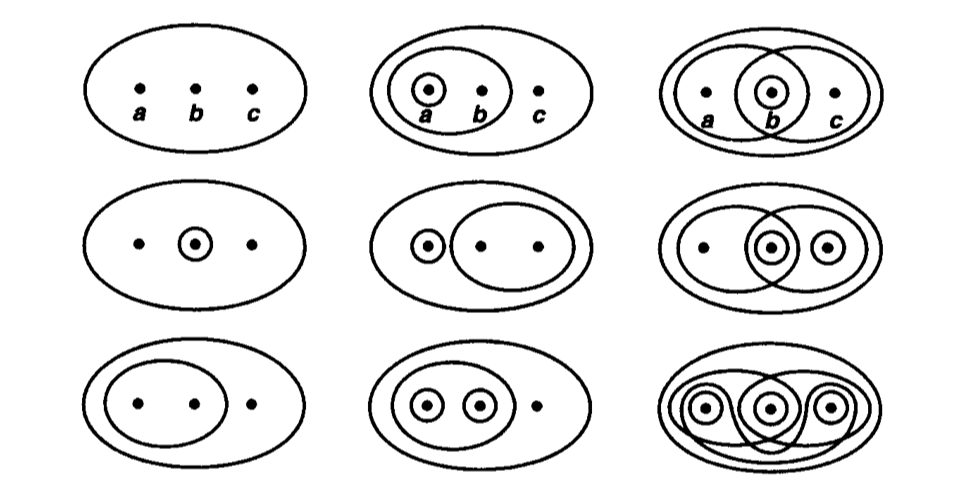
\includegraphics[scale=.75]{top_ex.png}
% 	\end{center}
% \end{figure}
% \end{exercise}
% \begin{solution}
% 	We'll label the examples by the coordinates $(i,j)$ where $i,j \in \{1,2,3\}$ correspond to the row/column number. Then, in the matrix below, we'll list which pair is finer, or ``inc'' if the pair is incomparable. 
% 	\begin{center}
% 	\begin{tabular}{ |c|c|c|c|c|c|c|c|c|c| } 	
% 		\hline
% 		& (1,1) & (1,2) & (1,3) & (2,1) & (2,2) & (2,3) & (3,1) & (3,2) & (3,3) \\	
% 		\hline
% 		(1,1) & = & (1,2) & (1,3) & (2,1) & (2,2) & (2,3) & (3,1) & (3,2) & (3,3) \\
% 		\hline 
% 		(1,2) & & = & inc & inc & inc & inc & (1,2) & (3,2) & (3,3) \\
% 		\hline
% 		(1,3) & & & = & (1,3) & inc & (2,3) & (1,3) & inc & (3,3) \\
% 		\hline
% 		(2,1) & & & & = & inc & (2,3) & inc & (3,2) & (3,3)\\
% 		\hline
% 		(2,2) & & & & & = & inc & inc & inc & (3,3) \\
% 		\hline
% 		(2,3) & & & & & & = & (2,3) & inc & (3,3) \\
% 		\hline
% 		(3,1) & & & & & & & = & (3,2) & (3,3) \\
% 		\hline
% 		(3,2) & & & & & & & & = & (3,3) \\
% 		\hline
% 		(3,3) & & & & & & & & & = \\ 
% 		\hline
% 	\end{tabular}
% 	\end{center}
% \end{solution}

% \begin{exercise}
% 	Show $\tT_c$ is a topology: Let $X$ be a set. Let $\tT_c$ be the collection of all subsets of $U$ of $X$ such that $X-U$ either is countable or is all of $X$. 
% \end{exercise}
% \begin{solution}
% 	We check the three conditions:
% 	\begin{enumerate}
% 		\item $X - \emptyset = X$ is all of $X$, so $\emptyset \in \tT_c$. $X - X = \emptyset$, which is finite, so $X \in \tT_c$.
% 		\item Let $\{U_\alpha\}$ be an indexed family of nonempty elements of $\tT_c$. Note that for each $\alpha$, $X - U_\alpha$ is countable. Then
% 		\begin{equation}
% 			X - \bigcup U_\alpha = \bigcap (X - U_\alpha)
% 		\end{equation}
% 		The intersection of countable sets is also countable, so $\{U_\alpha\} \in \tT_c$.
% 		\item Let $\{U_i\}_{i=1}^n$ be nonempty elements of $\tT_c$. Then
% 		\begin{equation}
% 			X - \bigcap_{i=1}^n U_i = \bigcup_{i=1}^n (X - U_i)
% 		\end{equation}
% 		The finite union of countable sets is also finite, so that $\{U_i\}_{i=1}^n \in \tT_c$.
% 	\end{enumerate}
% \end{solution}

% \begin{exercise}
% 	Is the collection $\tT_\infty = \{U | X-U \text{ is infinite or empty or all of $X$ } \}$ a topology on $X$?
% \end{exercise}
% \begin{solution}
% 	No. Counter example: 
% \end{solution}

\appendix

\section{Set Theory Review}

\begin{definition}[Difference]
	The \navy{difference} of two sets, denoted $A-B$, is the set consisting of those elements of $A$ that are not in $B$. In notation
	\begin{equation*}
		A - B = \{x | x \in A \text{ and } x \not\in B\}	
	\end{equation*}
\end{definition}

\begin{theorem}[Set-Theoretic Rules]
	We have that, for any sets $A, B, C$,
	\begin{enumerate}
		\item First distributive law for the operations $\cap$ and $\cup$:
		\begin{equation}
			A \cap (B \cup C) = (A \cap B) \cup (A \cap C)
		\end{equation}
		\item Second distributive law for the operations $\cap$ and $\cup$:
		\begin{equation}
			A \cup (B \cap C) = (A \cup B) \cap (A \cup C)
		\end{equation}
		\item DeMorgan's laws:
		\begin{equation}
			A - (B \cup C) = (A - B) \cap (A - C)
		\end{equation}
		``The complement of the union equals the intersection of the complements.''
		\begin{equation}
			A - (B \cap C) = (A - B) \cup (A - C)
		\end{equation}
		``The complement of the intersection equals the union of the complements.''
	\end{enumerate}
\end{theorem}

\subsection{Functions}

\begin{exercise}
 Let $f : A \to B$. Let $A_0 \subset A$ and $B_0 \subset B$. Then
 \begin{enumerate}
  	\item $A_0 \subset \inv{f}(f(A_0))$ and equality holds if $f$ is injective.
  	\item $f(\inv{f}(B_0)) \subset B_0$ and equality holds if $f$ is surjective.
  \end{enumerate} 
\end{exercise}
\begin{solution} We prove each item in turn:
\begin{enumerate}
	\item Let $a \in A_0$. Then $f(a) \in f(A_0)$. We have that $\inv{f}(f(A_0)) = \Set{a;f(a) \in f(A_0)}$. Then $f(a) \in \inv{f}(f(A_0))$, so that $A_0 \subset \inv{f}(f(A_0))$. We can actually show equality holds if and only if $f$ is injective. 
	\begin{enumerate}
		\item $\pmi$ Suppose $f$ is injective. Let $a \in \inv{f}(f(A_0))$. Then $f(a) \in f(A_0)$. Therefore there exists some $b \in f(A_0)$ such that $f(a) = f(b)$. Injectivity implies $a=b \in A_0$. 
		\item $\imp$ We will prove the contrapositive. Suppose $f$ is \emph{not} injective. Then $f(a) = f(b)$ for some $a \neq b$. Therefore $\Set{a,b} \subset \inv{f}(f(\Set{a}))$. Thus $\inv{f}(f(\Set{a})) \not\subset \Set{a}$.
	\end{enumerate}
	\item Let $x \in f(\inv{f}(B_0))$. Then there is some $b \in \inv{f}(B_0)$ such that $f(b) = x$. But $f(b) \in B_0$, so $x \in B_0$.
	\begin{enumerate}
		\item $\pmi$ Suppose $f$ is surjective. Take $b \in B_0$, then there exists some $a \in A_0$ such that $f(a) = b$, so that $a \in \inv{f}(B_0)$, and $b=f(a) \in f(\inv{f}(B_0))$. 
	\end{enumerate}
\end{enumerate}
\end{solution}

\begin{exercise}

\end{exercise}
\begin{solution}
\begin{enumerate}
	\item Let $B_0 \subset B_1$. Fix $x \in \inv{f}(B_0)$. Then $f(x) \in B_0$, which implies $f(x) \in B_1$. Thus $\inv{f}(B_0) \ss \inv{f}(B_1)$. 
	\item We show two inclusions:
	\begin{enumerate}
	 	\item $\supset$: We can use $(i)$, since $B_i \subset B_0 \cup B_1$, so $\inv{f}(B_0) \ss \inv{f}(B_0 \cup B_1)$ and $\inv{f}(B_1) \ss \inv{f}(B_0 \cup B_1)$, so $\inv{f}(B_0) \cup \inv{f}(B_1) \ss \inv{f}(B_0 \cup B_1)$.
	 	\item $\ss:$ Let $x \in \inv{f}(B_0 \cup B_1)$. Thus there exists some $b \in B_0 \cup B_1$ such that $f(x) = b$. Therefore $x \in \inv{f}(B_0)$ or $x \in \inv{f}(B_1)$, so that $\inv{f}(B_0 \cup B_1) \ss \inv{f}(B_1)$.
	 \end{enumerate}
	 \item  
\end{enumerate}
\end{solution}



\end{document}